\documentclass[11pt,a4paper]{article}

\usepackage{fontspec}
\setmainfont{Bitstream Charter}
\setsansfont{Latin Modern Sans}
\usepackage[a4paper,margin=2.3cm,headheight=22pt]{geometry}
\usepackage[table]{xcolor}
\definecolor{ink}{gray}{0.15}
\definecolor{rule}{gray}{0.75}
\definecolor{tint}{gray}{0.94}
\definecolor{link}{gray}{0.25}
\usepackage{booktabs,tabularx,array}
\usepackage{float,graphicx}
\usepackage{caption,subcaption}
\usepackage{amsmath,amssymb}
\usepackage{enumitem}
\usepackage{titlesec}
\usepackage{fancyhdr}
\usepackage{lastpage}
\usepackage[colorlinks=true,linkcolor=link,urlcolor=link,citecolor=link]{hyperref}

\AtBeginDocument{\color{ink}}
\setlist{itemsep=1pt,topsep=3pt,leftmargin=1.5em}
\setlength{\parindent}{0pt}
\setlength{\parskip}{5pt}
\renewcommand{\arraystretch}{1.2}
\arrayrulecolor{rule}
\heavyrulewidth=0.9pt
\lightrulewidth=0.4pt
\captionsetup{font={small,sf},labelfont=bf,labelsep=period,justification=raggedright,singlelinecheck=false}
\titleformat{\section}{\sffamily\large\bfseries}{\thesection}{0.6em}{}
\titleformat{\subsection}{\sffamily\normalsize\bfseries}{\thesubsection}{0.6em}{}
\titlespacing*{\section}{0pt}{14pt}{4pt}
\titlespacing*{\subsection}{0pt}{9pt}{3pt}

\pagestyle{fancy}
\fancyhf{}
\fancyhead[L]{\sffamily\small CSE558 Data Science \textbar\ Monsoon 2026}
\fancyhead[R]{\sffamily\small Project Proposal \textbar\ [Enter group name]}
\fancyfoot[C]{\sffamily\small\thepage\ / \pageref{LastPage}}
\renewcommand{\headrule}{\hbox to\headwidth{\color{rule}\leaders\hrule height 0.4pt\hfill}}

\newcommand{\code}[1]{{\small\ttfamily #1}}
\newcommand{\takeaway}[1]{\textbf{#1}}
\newcommand{\seedvalue}{\textbf{558}}
\newcommand{\stripe}{\rowcolors{2}{tint}{white}}
\hypersetup{pdftitle={Education, Sex, and Income in the UCI Adult Dataset}}

\begin{document}

\begin{center}
  {\sffamily\LARGE\bfseries Education, Sex, and Income in the UCI Adult Dataset}\\[5pt]
  {\sffamily\small Group: [Enter group name] \quad\textbar\quad TA mentor: [Enter name]}\\[2pt]
  {\sffamily\small Members: [Enter member names and roll numbers]}
\end{center}
\vspace{-4pt}
{\color{rule}\hrule height 0.6pt}
\vspace{6pt}

\section{Dataset}

We use the Adult dataset, extracted from the 1994 US Census database and
retrieved on 29 September 2026 from the official UCI archive
\cite{adult}. It contains \textbf{48,842 rows} and \textbf{15 columns}: 14
predictors and the binary target \code{income} (\code{>50K} or \code{<=50K}).
The predictors mix continuous, discrete, and nominal attributes. Age records
respondent age in years. \code{education-num} records an ordinal education
level, and \code{hours-per-week} records usual weekly work hours. Workclass,
occupation, sex, and race describe employment and demographic groups. The raw
files still contain \code{?} markers, exact duplicate records, and capital-gain
values top-coded at USD 99,999. We use this dataset because its mixed feature
types and documented data issues support both statistical inference and a
reproducible preparation study.

\begin{table}[H]
\centering\stripe
\caption{Selected attributes and their source meaning.}
\label{tab:selected-features}
\small
\begin{tabularx}{\textwidth}{@{}l l l X r@{}}
\toprule
\rowcolor{white}\textbf{Attribute} & \textbf{Type} & \textbf{Unit or range} & \textbf{Real-world meaning} & \textbf{Missing}\\
\midrule
\code{age} & discrete & years, 17--90 & Age of respondent & 0\%\\
\code{workclass} & nominal & 8 known levels & Employer type & 5.7\%\\
\code{education-num} & discrete & ordinal, 1--16 & Highest education level & 0\%\\
\code{occupation} & nominal & 14 known levels & Job category & 5.8\%\\
\code{capital-gain} & continuous & USD, 0--99,999 & Capital income; top-coded & 0\%\\
\code{hours-per-week} & continuous & hours, 1--99 & Usual weekly work hours & 0\%\\
\code{sex} & nominal & Female or Male & Recorded sex group; sensitive attribute & 0\%\\
\code{fnlwgt} & continuous & positive integer & Census sampling weight & 0\%\\
\bottomrule
\end{tabularx}
\end{table}

The target has 37,155 records at or below USD 50,000 (76.1\%) and 11,687 above
USD 50,000 (23.9\%). The full data dictionary appears in Appendix~\ref{app:dict}.

\subsection{Exploration and confirmation split}

We split before exploration and stratified on \code{income}. The exploration
partition contains \textbf{39,073 rows (80.0\%)} and the confirmation partition
contains \textbf{9,769 rows (20.0\%)}. The seed is \seedvalue, defined once in
\code{src/config.py}. All figures use exploration rows. Confirmation remains
closed until the hypothesis and analysis choices are fixed.

\clearpage
\section{Data preparation}

The table records proposed steps. The encoding and predictor choices have not
been applied to the full dataset or approved in the processing pipeline.

\begin{table}[H]
\centering\stripe
\caption{Proposed preparation decisions, alternatives, and quantified reasons.}
\label{tab:prep}
\footnotesize
\begin{tabularx}{\textwidth}{@{}>{\raggedright\arraybackslash}p{2.6cm} >{\raggedright\arraybackslash}p{3cm} >{\raggedright\arraybackslash}p{2.5cm} X@{}}
\toprule
\rowcolor{white}\textbf{Issue} & \textbf{Proposed step} & \textbf{Alternative} & \textbf{Reason}\\
\midrule
Missing values (\code{?}) & Convert to missing, then retain an explicit unknown category & Drop rows or impute the mode & The source has 6,465 marker cells: 2,799 in workclass, 2,809 in occupation, and 857 in native-country. An unknown category preserves records and keeps missingness visible.\\
Duplicate rows & Retain exact duplicates & Drop repeated rows & Exploration contains 38 exact duplicates among 39,073 records. No record identifier shows they are errors, so dropping them would alter observed frequencies.\\
Capital-gain top-code & Keep and flag USD 99,999 & Delete or winsorize capped values & There are 194 capped observations in exploration. The cap is a source limit, not evidence of invalid records.\\
Redundant education fields & Keep ordinal \code{education-num}; omit \code{education} from the candidate model matrix & Include both fields & The 16 education labels map one-to-one to numeric levels in exploration, with 0 mapping conflicts. Including both repeats the same information.\\
\code{fnlwgt} & Exclude it as a personal predictor & Treat it as an individual attribute & \code{fnlwgt} is a census sampling weight, not a personal characteristic. Any population-weighted inference needs a separate review of the weighting design.\\
Encoding & Candidate: one-hot encode 7 nominal fields and retain 5 numeric or ordinal fields; use an explicit missing category & Integer-code nominal values & The candidate has 91 columns and 4,444,622 cells over 48,842 rows, above the 3,000,000 floor. Integer codes would impose an order on nominal categories. This encoding has not been applied.\\
\bottomrule
\end{tabularx}
\end{table}

\section{Effect of preparation}

\begin{table}[H]
\centering\stripe
\caption{Projected effect of the proposed preparation. Duplicate counts refer to exploration only.}
\label{tab:effect}
\small
\begin{tabular}{@{}lrrr@{}}
\toprule
\rowcolor{white}\textbf{Metric} & \textbf{Before} & \textbf{Proposed after} & \textbf{Change}\\
\midrule
Rows & 48,842 & 48,842 & 0\\
Predictor or encoded feature columns & 14 & 91 & +77\\
Missing-marker cells & 6,465 & 0 & $-6,465$\\
Exact duplicates in exploration & 38 & 38 & 0\\
Share with income above USD 50,000 & 23.9\% & 23.9\% & 0.0 points\\
\midrule
Samples $\times$ features & 683,788 & 4,444,622 & $\ge 3{,}000{,}000$: yes\\
\bottomrule
\end{tabular}
\end{table}

The after column projects the proposed design. It is not a measured full-dataset
processed artifact. The duplicate count covers the exploration portion because
confirmation records remain closed. The proposal removes no rows. It omits two
raw predictors from the candidate model matrix: the redundant \code{education}
field and the sampling-weight field \code{fnlwgt}. It gains explicit missing
categories and one column per nominal category. Source top-coding means the
true capital-gain values above USD 99,999 cannot be recovered.

\section{Exploratory analysis}

\begin{figure}[H]
\centering
\begin{subfigure}[t]{0.98\textwidth}
  \centering
  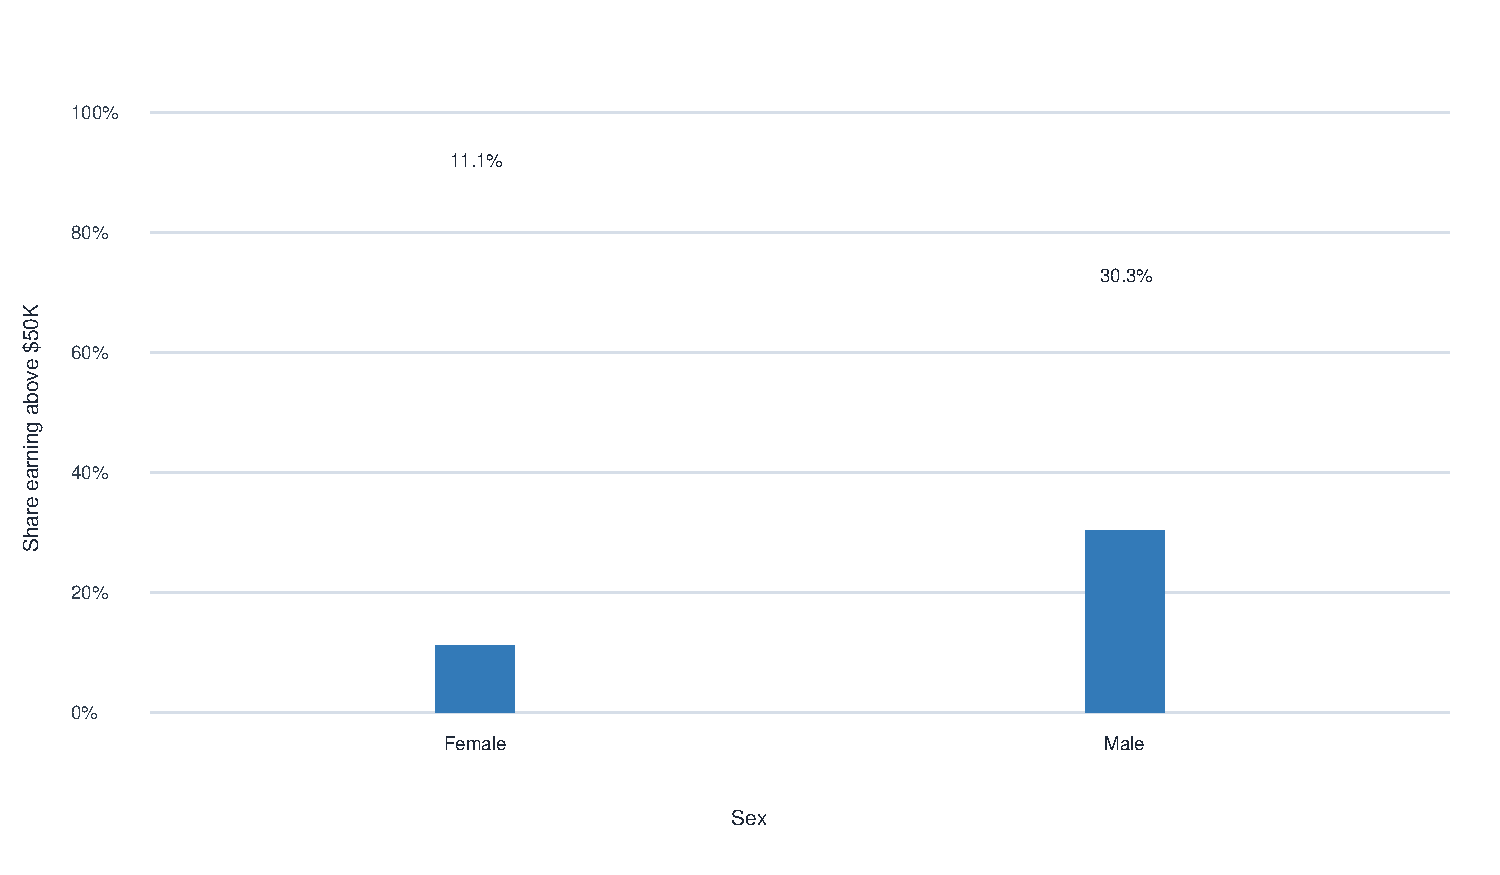
\includegraphics[width=\linewidth]{../reports/figures/income_by_sex.pdf}
  \caption{\takeaway{The exploratory above-USD-50,000 rate is 19.1 percentage points higher for males.} The rates are 30.3\% (7,908/26,132) for males and 11.1\% (1,441/12,941) for females.}
\end{subfigure}\\[4pt]
\begin{subfigure}[t]{0.98\textwidth}
  \centering
  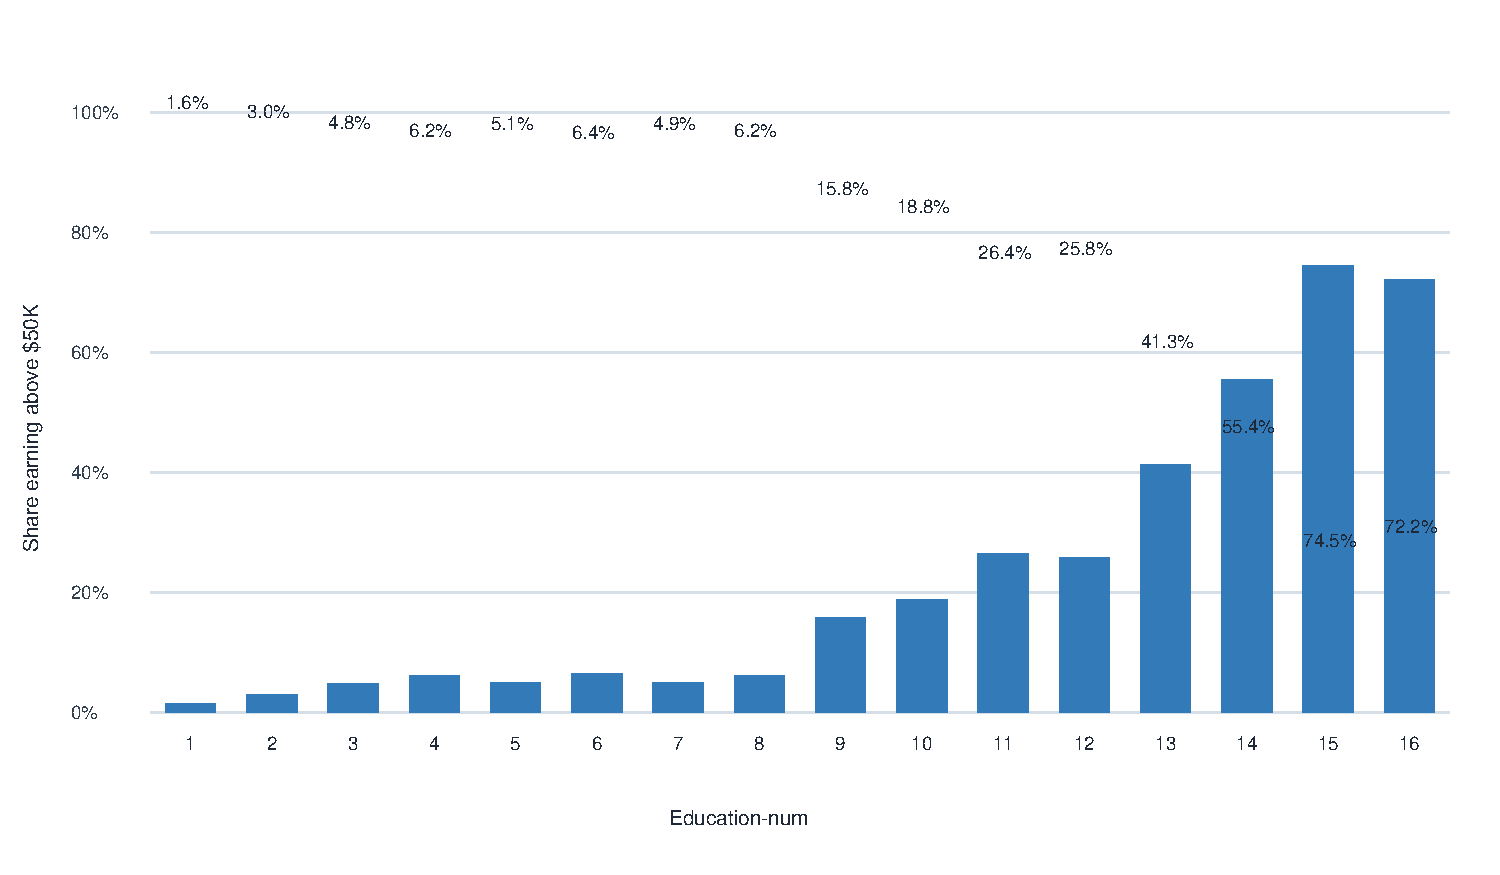
\includegraphics[width=\linewidth]{../reports/figures/income_by_education_num.pdf}
  \caption{\takeaway{The above-USD-50,000 rate spans 72.9 percentage points across education levels.} It ranges from 1.6\% at level 1 (1/64) to 74.5\% at level 15 (493/662).}
\end{subfigure}
\caption{Exploratory marginal rates motivate the proposed adjusted education-by-sex interaction analysis. These rates do not estimate adjusted effects.}
\label{fig:eda}
\end{figure}

\subsection{Obvious questions}

Anyone familiar with this dataset would ask:
\begin{enumerate}[label=\textbf{O\arabic*.},leftmargin=2.4em]
  \item Does income vary by education level?
  \item Does the income distribution differ by sex?
  \item Does income vary with hours worked per week?
\end{enumerate}

\subsection{Problem statement}

\begin{enumerate}[label=\textbf{P\arabic*.},leftmargin=2.4em]
  \item \textbf{Primary.} Does the association between \code{education-num} and income above USD 50,000 differ by sex? We will estimate it after adjusting for age and hours worked per week.
\end{enumerate}

\textbf{Why P1 is not on the obvious list.} P1 asks whether the education association differs by sex after adjustment for age and work hours. The obvious questions ask only about marginal patterns. We will make one confirmatory claim to avoid unnecessary multiple testing.

\subsection{Proposed inference}

We will fit logistic regression with income above USD 50,000 as the binary
outcome. Predictors will include education-num, sex, age, hours-per-week, and
the education-num-by-sex interaction. The null hypothesis is that the
interaction coefficient equals zero. The alternative is that it differs from
zero. We will compare nested models with a one-degree-of-freedom likelihood
ratio test and report the interaction estimate with a confidence interval.

This test assumes independent records, convergence, adequate cell counts, and
linear effects of continuous terms on the log-odds. We will check convergence,
sparse levels, and logit linearity. We will compare the result with a model
that treats education-num as categorical and tests a 15-degree-of-freedom
interaction. That alternative relaxes the linear education trend but uses more
parameters. It is an assumption check, not a second confirmatory claim. No
multiple-test correction is needed for one primary test; if later analyses add
confirmatory tests, we will use Holm correction.

Sex, race, and native-country are sensitive attributes. We will report group
counts and uncertainty and examine group differences in missingness. The
observational data support association claims only. A causal claim about
education would require a defensible causal design, temporal ordering, and a
strategy for confounding. Group rate differences alone do not establish
unfair treatment or measure fairness completely.

\section{Reproducibility}

The environment uses \code{uv}, \code{pyproject.toml}, and \code{uv.lock}. The
split seed is \seedvalue, and the raw archive remains unchanged. Run
\code{uv run python -m src.data.prepare} to recreate the split and
\code{uv run python -m src.analysis.explore} to regenerate the two proposal
figures. The archive SHA-256 is
\texttt{7537312d\allowbreak d56c2b98\allowbreak 03580805\allowbreak ce99e681\allowbreak 83a30ee4\allowbreak 685aa532\allowbreak 9d6df0fb\allowbreak b3cc21bb}.
Project repository: \url{https://github.com/durgesh-k-sharma/cse558-adult-project}.

\begin{thebibliography}{9}\small
\bibitem{adult} B.~Becker and R.~Kohavi. \emph{Adult}. UCI Machine Learning Repository, 1996.
\url{https://doi.org/10.24432/C5XW20}.
\end{thebibliography}

\clearpage
\appendix
\section{Data dictionary}\label{app:dict}

The missingness column reports source \code{?} markers before cleaning.

\begin{table}[H]
\centering\stripe
\scriptsize
\begin{tabularx}{\textwidth}{@{}l l l X r@{}}
\toprule
\rowcolor{white}\textbf{Attribute} & \textbf{Type} & \textbf{Unit or range} & \textbf{Meaning or values} & \textbf{Missing}\\
\midrule
\code{age} & discrete & years, 17--90 & Respondent age & 0\\
\code{workclass} & nominal & 8 categories & Employment class & 2,799 (5.7\%)\\
\code{fnlwgt} & continuous & positive integer & Census sampling weight & 0\\
\code{education} & nominal & 16 categories & Highest education category & 0\\
\code{education-num} & discrete & 1--16 & Ordinal education level & 0\\
\code{marital-status} & nominal & 7 categories & Marital status & 0\\
\code{occupation} & nominal & 14 categories & Occupation class & 2,809 (5.8\%)\\
\code{relationship} & nominal & 6 categories & Household relationship & 0\\
\code{race} & nominal & 5 categories & Recorded race; sensitive attribute & 0\\
\code{sex} & nominal & 2 categories & Female or Male; sensitive attribute & 0\\
\code{capital-gain} & continuous & USD, 0--99,999 & Capital gain; upper value is top-coded & 0\\
\code{capital-loss} & continuous & USD, 0--4,356 & Capital loss & 0\\
\code{hours-per-week} & continuous & hours, 1--99 & Usual weekly work hours & 0\\
\code{native-country} & nominal & 41 categories & Country of origin; sensitive attribute & 857 (1.8\%)\\
\code{income} & nominal & $\le$USD 50,000 or $>$USD 50,000 & Income bracket; target & 0\\
\bottomrule
\end{tabularx}
\end{table}

\end{document}
